\chapter{Ultrasound and its Challenges in GBC Detection}
\label{chap:usg}
%
Ultrasound (USG), a non-invasive medical imaging technique, employs high-frequency sound waves to create real-time visualizations of internal body structures. 
%One commonly used mode is B-mode, or brightness mode, which produces two-dimensional images by interpreting the echoes of sound waves bouncing off tissues. B-mode ultrasound is invaluable for assessing organ structure and detecting abnormalities. 
Unlike X-rays, USG does not involve the use of ionizing radiation, which makes it safe for a wide range of patients. In this chapter, we provide a concise overview of USG fundamentals, followed by an exploration of the unique challenges encountered in automated GBC detection using USG. By delving into these intricacies, readers will gain a deeper understanding of the problem.
%we briefly discuss the basics of USG, and then describe the challenges posed by USG in automated GBC detection, providing the reader the necessary details for better understanding.

\section{Basics of Ultrasound}
%
\subsection{Ultrasound Physics}
Sound is a series of pressure waves that propagate through a compressible medium. A single \emph{cycle} of a sound wave encompasses a complete positive and negative pressure change. The \emph{wavelength} is defined as the distance covered during one complete cycle. The \emph{frequency} of the wave is measured in cycles per second, denoted as Hertz (Hz). The strength or the level of the pressure is called \emph{amplitude}. The audible range of sound for humans is 20 Hz to 20 kHz. Ultrasound refers to sound waves with frequencies higher than 20 kHz. In diagnostic ultrasound, frequencies between 1--20 MHz are commonly used.

Ultrasound wave production and interpretation rely on the `pulse-echo principle.' The process begins with the piezoelectric crystal within the transducer, acting as the source of ultrasound waves. This crystal has the capability to convert electrical current into mechanical pressure waves (ultrasound waves) and vice versa. Following the generation of the ultrasound wave, the crystal shifts from `sending' to `listening' mode, anticipating the return of ultrasound echoes. Notably, transducers spend almost all their time in the `listening' mode. The ultrasound waves can move through the tissues in both longitudinal and transverse directions. 
The sending and receiving cycle repeats a few million times per second, forming the foundation for creating images on the ultrasound monitor. The resulting images are contingent on the direction, timing, and amplitude of the returning waves.
Understanding the relationship between ultrasound frequency and image resolution is pivotal in selecting the appropriate probes and frequencies. Lower frequencies can penetrate deeper into tissue but provide poorer resolution for fine detail. Conversely, higher frequency ultrasound offers more detailed images with superior resolution but sacrifices depth penetration. This nuanced understanding is crucial for optimizing image quality and extracting meaningful diagnostic information.

\subsection{Common Modes of USG}
%
%\mypara{A-mode}
%
%In the amplitude mode (A-mode), the recording process captures the amplitude of the transducer voltage as a function to the round-trip travel time of an ultrasound pulse. A-mode operates by transmitting a single pulse through the body, with the pulse scattering back to the same transducer element. The recorded voltage amplitudes show a linear correlation to acoustic pressure amplitudes.

\mypara{B-mode}
%
B-mode, also known as `brightness mode,' offers structural information by representing different shades of gray in a two-dimensional image. The brightness in this mode is determined by the amplitude of returning echoes. Different echogenicities (brightness) are described as follows:
\begin{itemize}
    \item \emph{Anechoic:} Complete or near absence of returning sound waves, resulting in a black area.
    \item \emph{Hypoechoic:} Structure has very few echoes and appears darker than surrounding tissue.
    \item \emph{Hyperechoic/ Echogenic:} Large amplitude of returning echoes makes the structure appear brighter than surrounding tissue.
\end{itemize}
We show a sample B-mode USG along with the different brightness regions in \cref{fig:d_mode}.

\begin{figure}[!t]
\centering
	\begin{subfigure}[b]{0.32\linewidth}
	\centering
	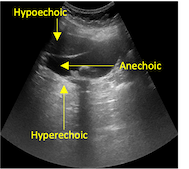
\includegraphics[width=\linewidth, height=8em]{figs/b_mode.png}
		\caption{}
		\label{fig:b_mode}
	\end{subfigure}
	%
	\begin{subfigure}[b]{0.32\linewidth}
	\centering
	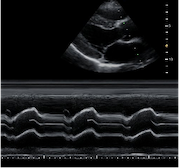
\includegraphics[width=\linewidth, height=8em]{figs/m_mode.png}
		\caption{}
		\label{fig:m_mode}
	\end{subfigure}
	%
        \begin{subfigure}[b]{0.32\linewidth}
	\centering
	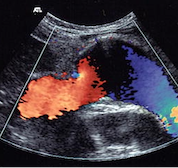
\includegraphics[width=\linewidth, height=8em]{figs/d_mode.png}
		\caption{}
		\label{fig:d_mode}
	\end{subfigure}
	\caption[Sample USG images from different modes]{Sample USG images from different modes. (a) B-mode, also highlights the anechoic, hypoechoic, and hyperechoic regions. (b) M-mode USG. (c) Doppler mode (color Doppler) USG.}
    \label{fig:usg_modes}
\end{figure}

\mypara{M-mode}
%
In motion mode, successive pulses are emitted. The backscattered signal is then converted into lines of bright pixels, where the brightness linearly correlates to backscattered voltage amplitudes. Each subsequent line is plotted adjacent to the previous one, producing an image resembling a B-mode image. This enables the visualization of movement in structures positioned along that line. A sample M-mode USG is shown in \cref{fig:m_mode}.

\mypara{Doppler mode}
%
Doppler mode involves analyzing the attributes of tissue motion and blood flow, including direction and speed. The core of this process relies on the `Doppler shift' phenomenon, which denotes the alteration in frequency between the transmitted and the returning sound wave. This technique is instrumental in capturing and interpreting the dynamic aspects of tissue motion and blood flow, providing valuable insights through various display modalities. \cref{fig:d_mode} shows a sample Doppler mode USG.
\begin{itemize}
    \item \emph{Color Doppler:} The direction and velocity of tissue motion and blood flow are color-coded and superimposed onto the corresponding B-mode image. 
    \item \emph{Power Doppler:} Captures the amplitudes of the returning frequency shifts onto the corresponding B-mode image. Typically used during vascular emrgencies with low flow state.
    \item \emph{Spectral Doppler:}  The spectrum of the Doppler frequencies returning to the transducer are Fourier transformed, and presented in a continuous and pulse-wave form.
\end{itemize}

\begin{figure}[!t]
    \centering
    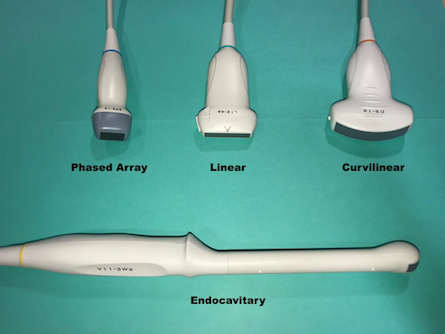
\includegraphics[width=0.5\linewidth]{figs/usg_probes.png}
    \caption[Common USG probes]{Four common types of probes used in diagnostic ultrasound imaging. Image courtesy: American College of Emergency Physicians \cite{acep}.}
    \label{fig:usg_probes}
\end{figure}

\subsection{Types of Probes}
%
Transducers or probes are comprised of three main components: the active element, which is typically a piezoelectric crystal, a damping material, and a matching layer. The arrangement of the active element can take various forms, resulting in a variety of probe configurations. Following are few of the most commonly used probe types,
\begin{enumerate}
    \item \textbf{Curvilinear (Curved Array):} This type of probe has a large curved footprint. The curved array probes produce images with shape resembling to the sector of a circle. These probes operate on low frequency, and are primarily employed for transabdominal ultrasound. 
    %
    \item \textbf{Phased Array:} This transducer produces a sector-shaped image with a smaller footprint, making it ideal for use between ribs. It operates at a low frequency and is primarily employed in cardiac and transabdominal ultrasound.
    %
    \item \textbf{Linear:} This transducer generates a rectangular image with a straight, flat footprint and is characterized by a high frequency. Its primary applications include vascular ultrasound, procedural guidance, and the assessment of superficial soft tissue structures.
    %
    \item \textbf{Endocavitary:} This transducer has a small curved footprint, and operates at a medium frequency. These are primarily used for endovaginal or intraoral ultrasound.
\end{enumerate}
\cref{fig:usg_probes} shows the curvilinear and the other commonly used probes.

\subsection{Body Planes}
%
\begin{figure}[!ht]
    \centering
    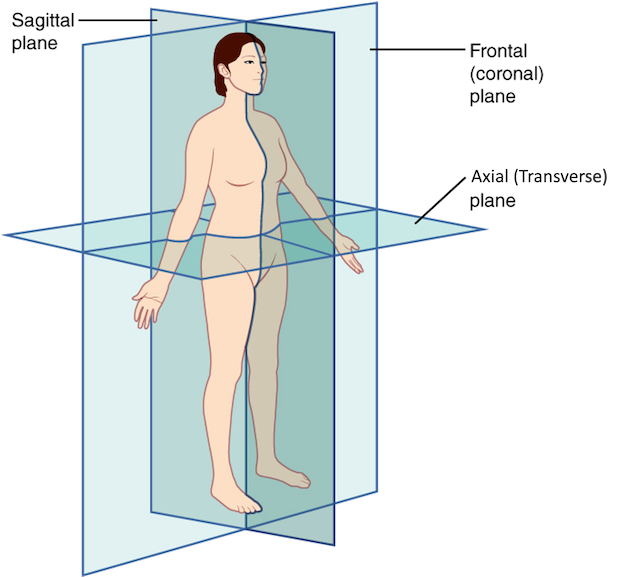
\includegraphics[width=0.5\linewidth]{figs/body_planes.png}
    \caption[Different body planes for radiological scanning]{The three different body planes relevant for scanning in radiology. Image courtesy: Wikipedia \cite{body_plane}.}
    \label{fig:body_plane}
\end{figure}
The \textbf{sagittal plane} is oriented perpendicular to the ground, distinguishing the left from the right, when an individual is in a \emph{supine position}. In supine position, a person lies on their back with the face and torso facing upwards.

The \textbf{axial plane}, also called the \textbf{transverse plane} or cross-sectional plane, is positioned perpendicular to the ground when the patient is in a supine posture. It differentiates the superior from the inferior or the head from the feet.

In the supine position, the \textbf{frontal plane}, also known as the coronal plane, aligns parallel to the ground, distinguishing the anterior from the posterior or the front from the back.

The illustration in \cref{fig:body_plane} depicts the three distinct body planes that are pertinent for scanning in radiology.

In addition to the three standard scanning planes, an \textbf{oblique plane} may also be used by the radiologist. As the name suggests, oblique plane is any plane which is not parallel or not in right angle to any of sagittal, axial, and frontal planes.

% \subsection{Probe Movements}
% %
% In ultrasound imaging, various movements of the probe are employed for effective examination \cite{bahner2016language}:

% \begin{itemize}
 
%     \item \textbf{Slide:} This involves moving the probe in the long axis along the surface of the body. The probe remains perpendicular to the target.

%     \item \textbf{Sweep:} This entails moving the probe in the short axis along the surface of the body. Similar to sliding, the probe remains perpendicular to the target.

%     \item \textbf{Rock:} In this movement, the probe travels along its long axis without changing the point of contact between the probe and the surface of the body.

%     \item \textbf{Fan:} The probe moves along its short axis without changing the point of contact between the probe and the surface of the body.

%     \item \textbf{Pressure:} This movement involves pushing the probe into the surface of the body. The footprint maintains contact with the surface, and the probe remains perpendicular to the target.

%     \item \textbf{Rotate:} The probe is rotated either clockwise or counterclockwise. The footprint maintains contact with the surface of the body, and the probe remains perpendicular to the target.
% \end{itemize}

\begin{figure}[!t]
\centering
    \begin{subfigure}[b]{0.32\linewidth}
    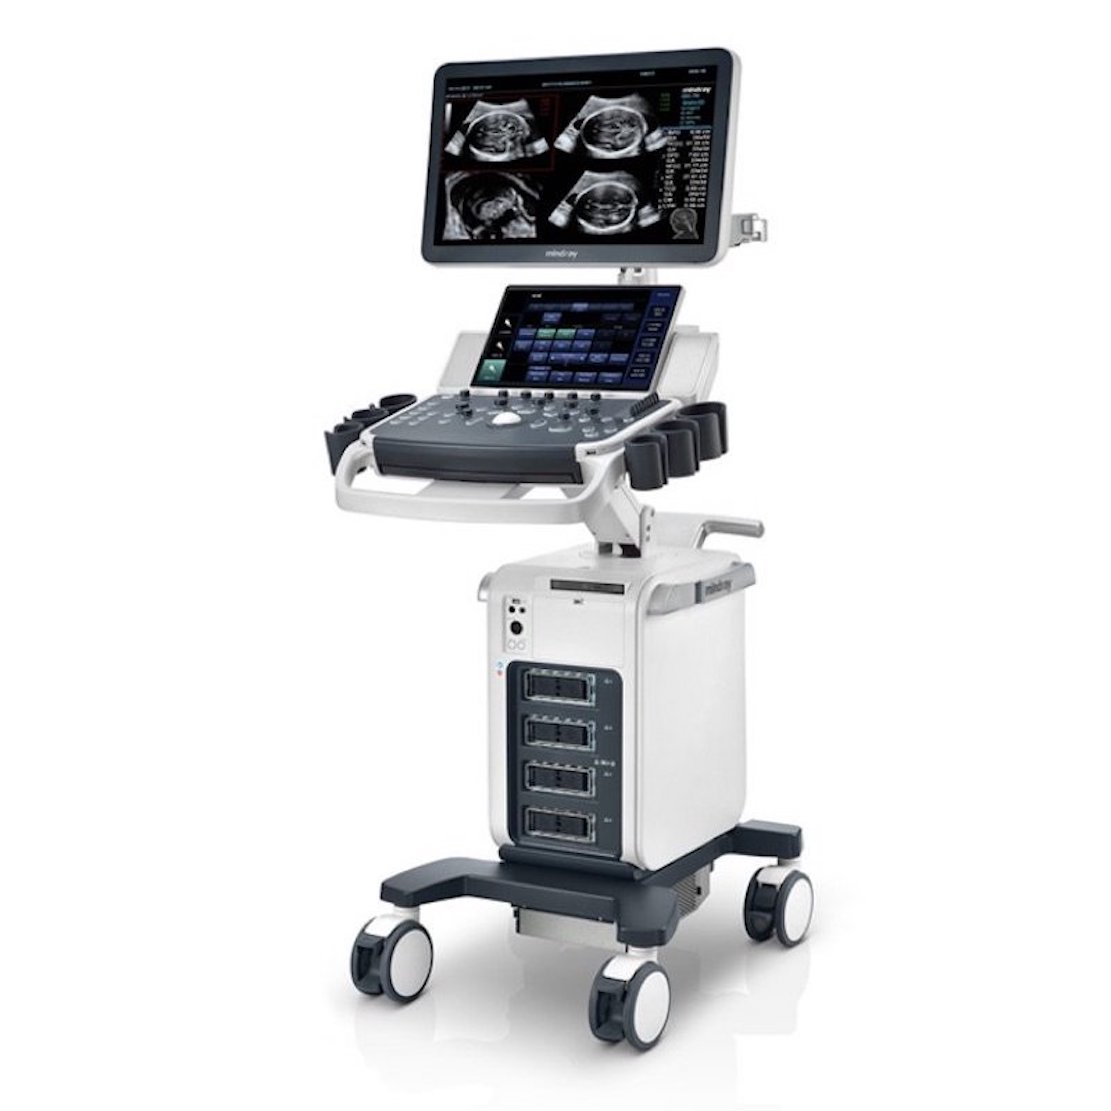
\includegraphics[width=\linewidth, height=8em]{figs/usg_machine.jpg}
    \caption{}
    \label{fig:usg_machine}
    \end{subfigure}
    %
    \begin{subfigure}[b]{0.24\linewidth}	
    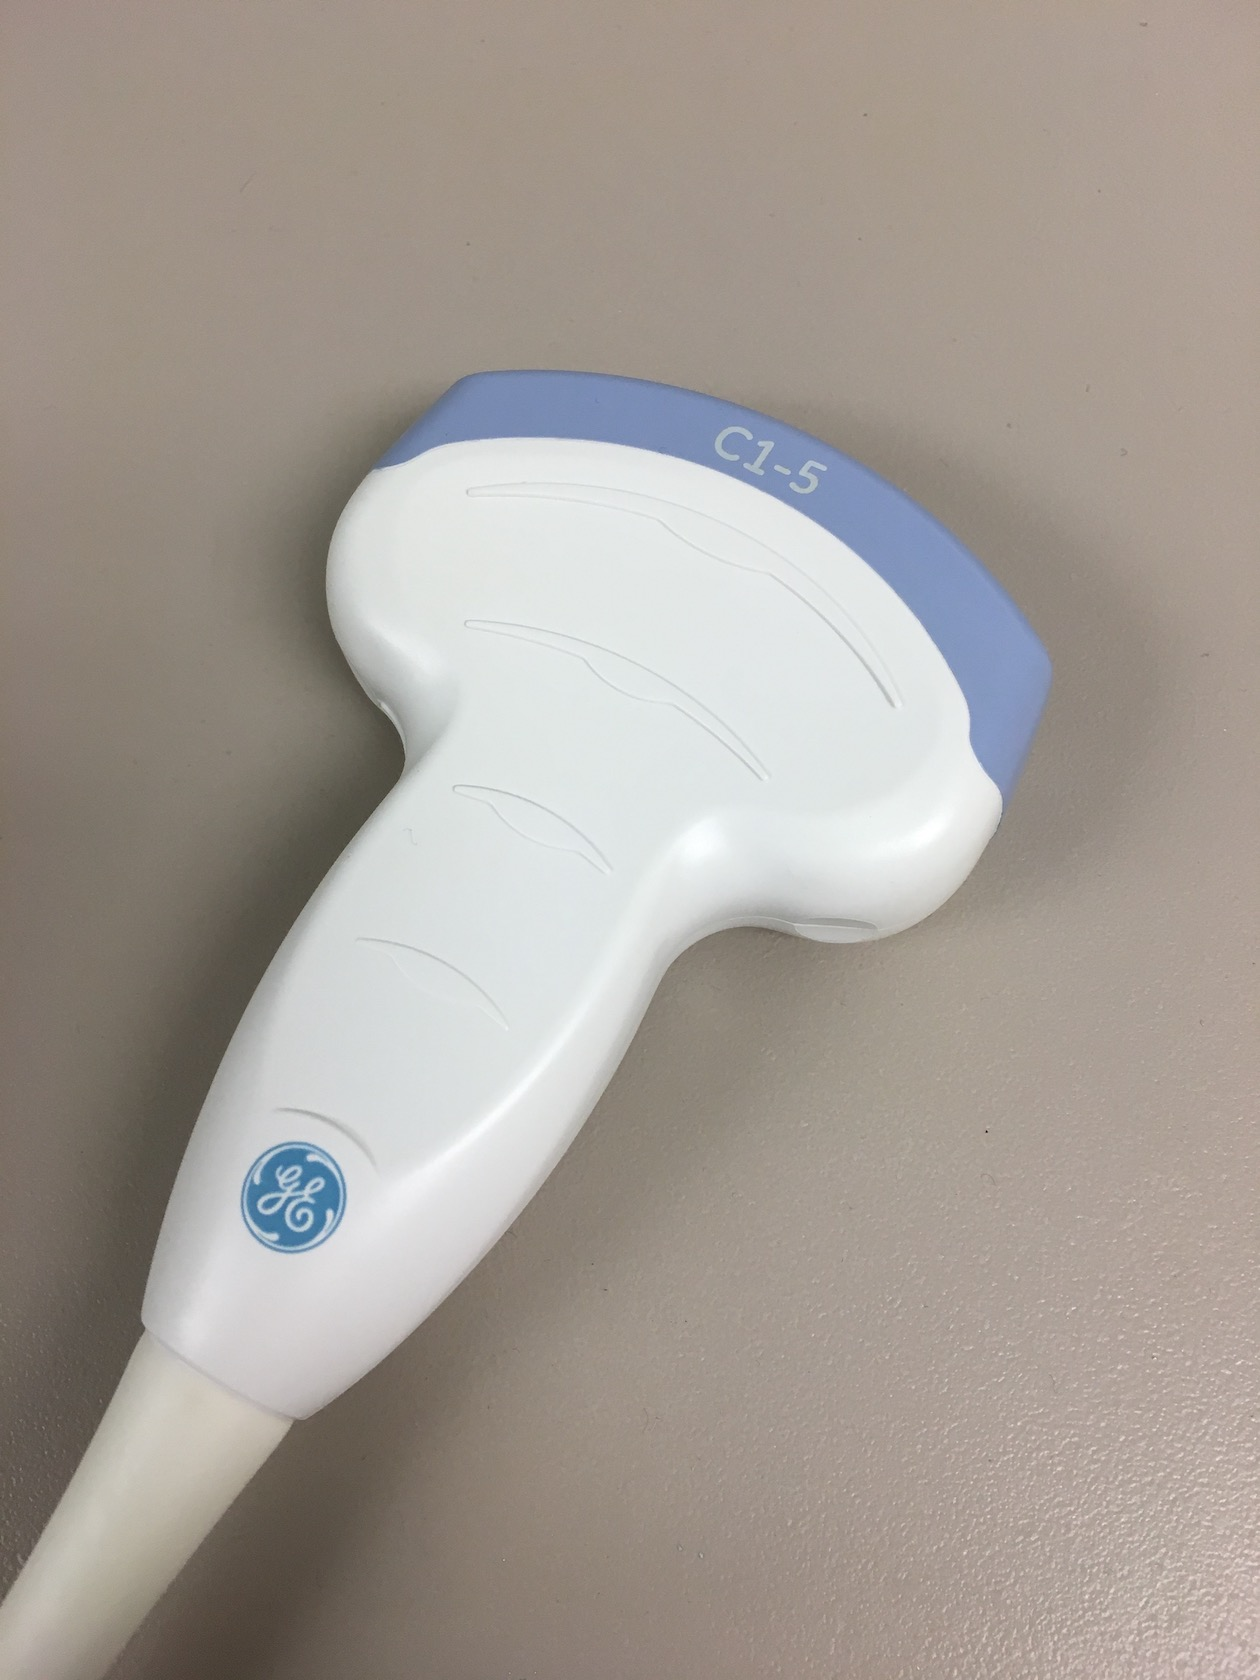
\includegraphics[width=\linewidth, height=8em]{figs/transducer.jpg}
    \caption{}
    \label{fig:usg_probe}
    \end{subfigure}
    %
    \begin{subfigure}[b]{0.32\linewidth}	
    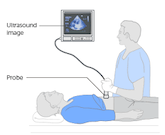
\includegraphics[width=\linewidth, height=8em]{figs/usg_overall.png}
    \caption{}
    \label{fig:usg_diag}
    \end{subfigure}
    \caption[Ultrasound machine, probe, and schematic diagram of abdominal USG]{(a) An USG machine with the display on top, control panel in the middle, and the computing engine on the base. (b) A curvilinear transducer (also called probe or sensor) commonly used for abdominal USG. (c) Schematic diagram of the USG procedure. Image courtesy: Cancer UK \cite{usg_diag}.}
    \label{fig:sample_usg}
\end{figure}

\section{Brief Description of Abdominal USG}
%
Abdominal USG focuses on scanning the organs within the abdominal cavity. It provides detailed views of the liver, kidneys, gallbladder, pancreas, and other abdominal structures, aiding in diagnosing conditions such as liver disease, kidney stones, or gallbladder ailments.

\par The USG scanning procedure involves applying a gel to the patient's skin to facilitate sound wave transmission and then using a transducer to emit and receive the waves. The resulting images guide healthcare professionals in making accurate diagnoses without the need for invasive procedures. Usually a handheld curved array probe is used for abdominal USG. The probe serves as both an emitter and receiver of sound waves. When the waves encounter different tissue densities, they reflect back to the transducer at varying speeds, forming a detailed image on the monitor. Radiologists strategically position the transducer on the patient's skin, manipulating its orientation and depth to capture comprehensive views of the targeted area. \cref{fig:usg_diag} shows a schematic diagram of the scanning process and the transducer probe.
Overall, USG combines sophisticated technology with skilled operator expertise to provide detailed, real-time images that aid in the affordable and safe diagnosis and monitoring of various medical conditions.

\section{Brief Specification of Our Data}
%
We have collected patient data from the Radiology department of a tertiary care apex hospital in Northern India. Patients were scanned using a Logiq S8 (GE Healthcare) machine with a low-frequency curvilinear probe (C1-5-D) operating at a frequency of 1-5 MHz in B-mode ultrasound. We have curated image data for 218 patients (1155 images), and video data for 73 patients (91 videos). We obtained written patient consent, and anonymized the data to protect patient privacy as per Ethics committee guidelines. Ultrasound scans were captured from different views and scanning planes to ensure adequate visualization of the pathology. 
In \Cref{chap:data} we provide more details regarding the dataset collection, annotation, and data statistics. In the following sections in this chapter, we outline the noise and artifacts in abdominal USG, the challenges of detecting GBC from USG, and also the specific issues pertaining to our data.

%\subsection{Applications of USG}
%
\section{Noise and Artifacts in Abdominal Ultrasound}
\label{sec:artifact_in_usg}

\begin{figure}[!t]
\centering
    % \begin{subfigure}[b]{0.23\linewidth}
    % 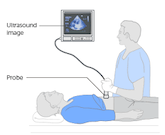
\includegraphics[width=\linewidth, height=6em]{figs/usg_overall.png}
    % \caption{}
    % \label{fig:usg_diag}
    % \end{subfigure}
	\begin{subfigure}[b]{0.24\linewidth}
	\centering
	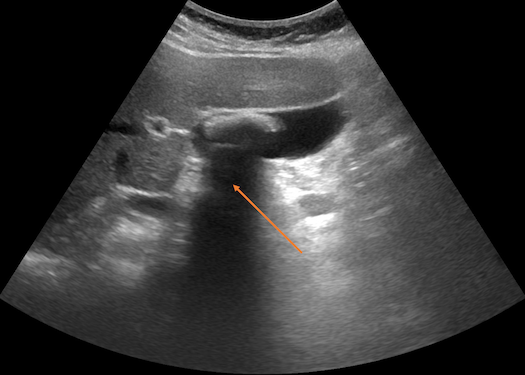
\includegraphics[width=\linewidth, height=7em]{figs/shadow.png}
		\caption{}
		\label{fig:usg_shadow}
	\end{subfigure}
	%
	\begin{subfigure}[b]{0.24\linewidth}
	\centering
	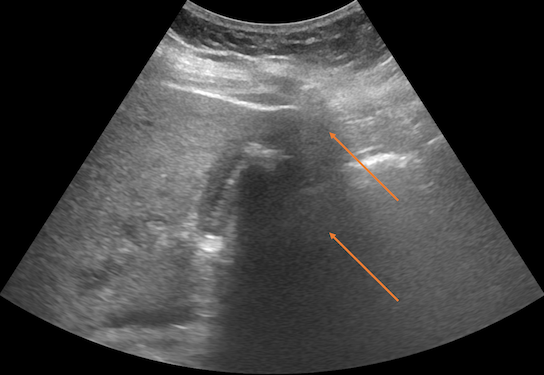
\includegraphics[width=\linewidth, height=7em]{figs/speckle.png}
		\caption{}
		\label{fig:usg_speckle}
	\end{subfigure}
	%
        \begin{subfigure}[b]{0.24\linewidth}
	\centering
	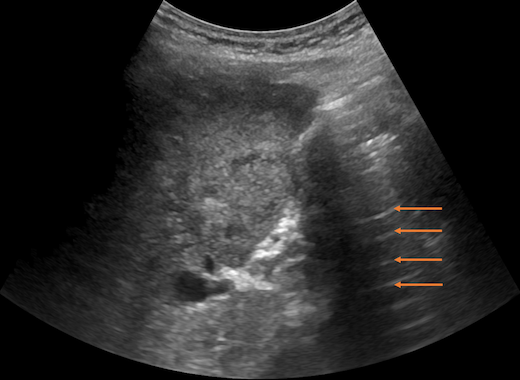
\includegraphics[width=\linewidth, height=7em]{figs/reverb.png}
		\caption{}
		\label{fig:usg_reverb}
	\end{subfigure}
    %
        \begin{subfigure}[b]{0.24\linewidth}
	\centering
	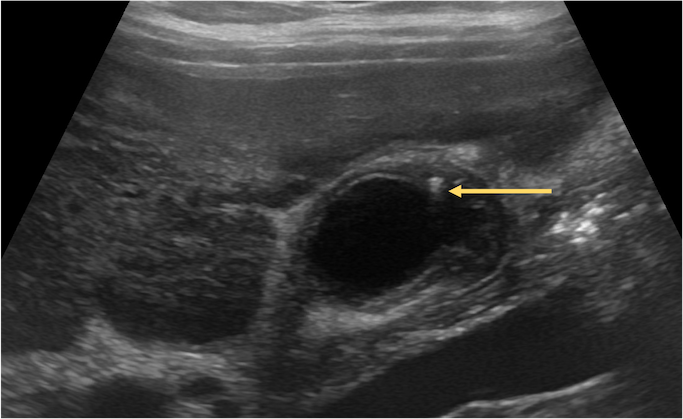
\includegraphics[width=\linewidth, height=7em]{figs/comet_tail.png}
		\caption{}
		\label{fig:usg_comet}
	\end{subfigure}
	\caption[Visualization of common artifacts present in our data]{Visualization of common artifacts present in our ultrasound dataset. (a) Ultrasound image sample showing the acoustic shadow artifacts caused by solid objects such as gallbladder stones. (b) Example of the speckle noise present in USG. (c) Reverberation artifact in ultrasound images. (d) Comet tail artifact in gallbladder. }
    \label{fig:sample_artifact_usg}
\end{figure}

%
In abdominal ultrasound imaging, various types of noise and artifacts can affect the quality and accuracy of the images produced. These artifacts may arise from factors such as equipment limitations, patient anatomy, or the interaction of sound waves with tissues. Understanding these artifacts is crucial for radiologists in interpreting ultrasound results. Such artifacts also influence the outcome of the DNN models. We briefly highlight some common types of artifacts found in ultrasound imaging, especially the ones our data manifested in this section. 

\mypara{Acoustic Shadows} This artifact occurs when sound waves encounter a strongly reflective or absorptive structure, leading to a shadow on the image. For example, bones or gallstones can cause acoustic shadowing, making it challenging to visualize structures behind them. \cref{fig:usg_shadow} shows a sample of the acoustic shadowing caused by a gallbladder stone. In our data, the acoustic shadows played a significant role in degrading the performance of popular off-the-shelf DNN models.
    
\mypara{Speckle Noise} A Speckle is a granular pattern that can appear on ultrasound images. It is a form of noise caused by interference patterns in the ultrasound beam. Speckle noise in inherent to ultrasound imaging, and is illustrated in \cref{fig:usg_speckle}. Our data samples also contained speckled noise. Advanced image processing techniques involving smoothing are usually employed to reduce the impact of speckle noise \cite{despeckle}. 
    
\mypara{Reverberation} Reverberation artifacts happen when sound waves bounce back and forth between two strong reflectors, creating multiple equally spaced lines on the image. This can create false echoes and distort the interpretation of structures. In our data, reverberation was another common artifact. \cref{fig:usg_reverb} presents an example of the reverberation artifacts from our dataset, highlighted with arrows. 
    
\mypara{Comet Tail Artifact} Similar to reverberation, a comet tail artifact is a dense line extending from a highly reflective structure. It is often seen behind gas bubbles or calcifications and may obscure the details of nearby structures. Some samples of our data demonstrated comet tail artifact. One such sample is shown in \cref{fig:usg_comet}. However, comet tail artifact is usually associated with benign GB pathology such as adenomyomatosis \cite{oh2019comet}, and is helpful for radiologists. 
    
%\mypara{Anisotropy} When ultrasound waves encounter a fibrillar structure, like a tendon or ligament, the fibrils can redirect a significant portion of the incoming sound beam away from the transducer. In such instances, the transducer does not capture the returning echo, leading it to interpret the insonated area as hypoechoic (darker than surrounding tissues). This happens because the majority of the reflected sound waves move away from the transducer, causing it to infer a reduced echogenicity (brightness of an area) in the imaged region. Anisotropy is usually manifested in Musculoskeletal ultrasound. 
    %
    %\item \mypara{Slice Thickness} This artifact occurs when the ultrasound beam has a finite thickness, causing structures to appear larger than they actually are. It can affect the accuracy of measurements and spatial resolution.
%

Understanding and recognizing these issues is essential to differentiate between genuine anatomical features and artifacts, ensuring accurate diagnosis and interpretation of ultrasound images. 

\section{Major Challenges}
\label{sec:challenges}
%% Expand the subsections -- some more elaboration
%
While identifying benign afflictions, such as stones, polyps, or GB wall thickening in routine USG is straightforward, accurate characterization and GBC detection is challenging for the radiologists \cite{gb-rads-paper, gupta2020imaging}. Our findings show that even the expert radiologists with 10 and 2 years of experience in abdominal radiology could only attain a sensitivity of about 70\% while detecting GBC from USG. In this section, we first describe the clinical challenges faced by radiologists, and then highlight the significant obstacles arising from noise, artifacts, and viewpoint variations in USG, which we encountered while applying DNN models to analyze USG images in this work. We have tackled issues including noise and artifacts such as acoustic shadows and bias to echogenic textures, small sized pathological regions, variation in appearance due to non-regular anatomy and operator bias, and low volume of data.  %These challenges and the solutions to remediate them are discussed in the subsequent chapters.

\begin{figure}[t]
    \centering
    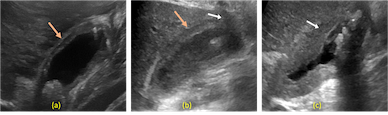
\includegraphics[width=0.8\linewidth, height=7em]{figs/clinical.png}
    \caption[Appearances of benign and malignant wall thickening]{(a) Shows a benign wall thickening with typical eco-layering (orange arrow). (b) Presents the wall thickening in a pathologically proven malignant GB. Notice the layered appearance (marked with the orange arrow) in this malignant thickening. Further, the thickening appears diffuse and symmetric, which is typically observed in benign cases. (c) Another pathologically proven case of GBC. Note that the wall thickening is more pronounced and irregular unlike the benign thickening.}
    \label{fig:clinical}
\end{figure}

\subsection{Challenges in Clinical Characterization of GB Wall Thickening}
\label{sec:clinical}
%
Clinical characterization of benign versus malignant GB wall thickening is challenging for even the experienced Radiologists due to multiple overlapping imaging features. Although GBC typically manifests asymmetric and irregular wall thickening, early stages of the disease may also manifest smooth and symmetric wall thickening, which is typical for benign conditions \cite{gupta2020imaging}. Additionally, as highlighted in \cref{fig:clinical}, traditional signs of benign thickening, like echo-layering (layered appearance) of the gallbladder wall, may also manifest in malignant cases, leading to diagnostic uncertainty. Furthermore, gallbladder wall thickening can occur in various conditions beyond GBC, such as acute cholecystitis, hepatitis, renal failure, pancreatitis, and Rokitansky-Aschoff sinuses \cite{gbc-lancet, gbc-xgc, gupta2020imaging}. The presence of these confounding factors can obscure the distinction between benign and malignant causes of wall thickening.
%the presence of various confounding factors, including systemic illnesses, can obscure the distinction between benign and malignant causes. As diagnostic criteria evolve, features once considered specific to benign conditions may be found in malignant cases as well, complicating interpretation. 
Ultimately, definitive diagnosis often requires histopathological evaluation to differentiate between benign and malignant pathologies conclusively, as radiologists often face difficulty in detecting GBC through non-invasive methods such as ultrasound. DNN methods can bridge this gap in non-invasive detection of GBC.

\begin{figure}[t]
    \centering
    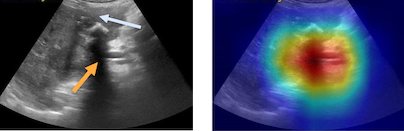
\includegraphics[width=0.8\linewidth]{figs/shadow_bias.png}
    \caption[Visualization of issues arising from artifacts such as acoustic shadow]{The black shadow (highlighted by the orange colored arrow) in the center of the left side image has visual similarities with the appearance of a normal \gb. The blue colored arrow shows the malignant region in the image. On the right side, we show the Grad-CAM \cite{gradcam} visual of a fine-tuned ResNet-50 \cite{resnet} model to visualize the salient region localized by the model. Clearly, the model is not accurately picking up the malignant regions, and is getting biased by the shadow region.}
    \label{fig:shadow_bias}
\end{figure}

\begin{figure}[t]
    \centering
    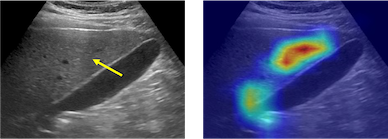
\includegraphics[width=0.8\linewidth, height=10em]{figs/texture_bias.png}
    \caption[Textures of liver tissues leading to incorrect GBC predictions]{The echogenicity of liver tissues resemble to gallbladder lesions/ masses. The adjacent liver tissue textures can bias the DNNs and lead to incorrectly predicting a normal gallbladder to be malignant. Liver is shown with yellow arrow in left image. On the right, we see from the Grad-CAM visual that Resnet-50 identifies the liver tissues as salient regions, and incorrectly predicts malignancy.}
    \label{fig:texture_bias}
\end{figure}

\begin{figure}[!ht]
    \centering
    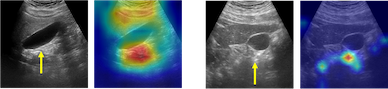
\includegraphics[width=0.8\linewidth]{figs/bright.png}
    \caption[Visualization of DNN models getting biased by hyperechoic regions]{The hyperechoic regions (highlighted by the yellow arrows) may bias the DNNs, and appear more distinctive over the GB regions to the networks. We show the Grad-CAM visual of a fine-tuned ResNet-50 model to identify the salient region localized by the model. The model is not accurately localizing the normal GB in these images, and instead focus on the bright regions.}
    \label{fig:hyperechoic_bias}
\end{figure}

\subsection{Low Image Quality -- Noise and Artifacts}
\label{sec:usg_artifact_issue}
%
% GBC detection from USG faces major challenges from low image quality, marked by noise, artifacts like shadows, and spurious textures. Unlike CT or MRI, USG suffers from low image quality arising from the noise and artifacts, as discussed previously in \cref{sec:artifact_in_usg}. Artifacts such as the shadows often show the visual traits of a non-malignant GB region, introducing bias to state-of-the-art DNN classifiers and resulting in suboptimal detection accuracy \cite{basu2022surpassing}. We present one such example in \cref{fig:shadow_bias}. The shadow region has a visual semblance with the appearance of the GB in ultrasound images. A finetuned Resnet-50 model identifies this region as a salient region, and results in incorrect prediction. 
% Additionally, The handheld nature of ultrasound sensors introduces operator-specific visual variations across radiologists and medical centers. These cause a large  The handheld nature of the sensor, and the operator-specific biases in view selection can result in radiologists selecting different frames from an USG scan (available in the form of a video) for assessment, introducing inter-observer variability. 

% Further, malignancy usually appears in a small part of the image, resulting in the low inter-class variability of the data. Also USG images are 2D slices of the 3D organs. The handheld nature of the probe causes large variation in different view points within the same patient, causing high intra-class variability. These issues make accurate prediction difficult for the DNN models. \cref{wsod_fig:variability_teaser} presents a depiction of the low inter-class and high intra-class variability.
Using DNNs to detect GBC from USG images presents formidable challenges arising from the inherent limitations in image quality. The USG modality, unlike CT or MRI, is susceptible to sensor artifacts, such as noise, shadows, and spurious textures. The low image quality arising from the sensor artifacts is a crucial factor complicating the accurate identification of malignant features in gallbladder regions, as discussed in \cref{sec:artifact_in_usg}. We further elaborate the specific challenges that we came across during the course of this work.

One notable challenge lies in artifacts like shadows or the anechoic regions, which often exhibit visual traits resembling non-malignant gallbladder regions. This introduces a bias to contemporary DNN classifiers, resulting in suboptimal detection accuracy \cite{basu2022surpassing}. A concrete example of this challenge is illustrated in \cref{fig:shadow_bias}, where a shadow region, sharing visual similarities with the gallbladder, is erroneously predicted as a salient region by a finetuned Resnet-50 model. 

The echogenic textures of the soft tissues of the organs such as liver often resemble the gallbladder lesions. Such textures appearing near the GB region can mislead a DNN model into falsely detecting malignancy. \cref{fig:texture_bias} demonstrates such an event of the model identifying the liver tissue as the salient region, and incorrectly predicting the sample to be malignant.

Additionally, standard DNNs may also get biased by the bright or hyperechoic regions, as these regions could appear distinctive to the networks. \cref{fig:hyperechoic_bias} shows an example of a Resnet-50 model focusing on the region with increased echogenicity. 



\subsection{Handheld Transducer -- Viewpoint and Operator Variability}
%
The handheld nature of ultrasound transducers (probes) adds another layer of complexity. It introduces operator-specific visual variations across different radiologists and medical centers, contributing to inter-observer variability. 
We further note that USG images provide 2D slices of 3D organs. Thus the angle of the transducer can significantly influence the appearance of the GB, and cause substantial variation in viewpoints within the same patient. Due to the change in the angle of insonation, some artifacts resembling the polypoidal mass can be observed in an otherwise normal gallbladder. \Cref{fig:angle_pseudo} presents an example of how changing the view from sagittal to axial leads to the pseudo-appearance of an artifact. 

\begin{figure}[t]
    \centering
    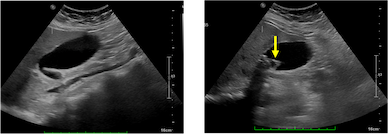
\includegraphics[width=0.6\linewidth, height=8em]{figs/angle_pseudo.png}
    \caption[Angle of transducer causing pseudo structures]{Sagittal (on left) and axial (on right) views of the gallbladder in a patient. On sagittal view, the GB wall is uniformly smooth and normal. The axial images gives a false appearance of the polypoidal mass arising from the gallbladder wall. This pseudo-appearance is due to the angle of insonation, and causes incorrect diagnosis.}
    \label{fig:angle_pseudo}
\end{figure}

\begin{figure}[!ht]
    \centering
    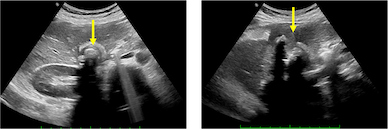
\includegraphics[width=0.6\linewidth, height=8em]{figs/oblique_thickening.png}
    \caption[Viewpoint variation leading to incorrect diagnosis]{True axial (on left) and Oblique axial (on right) views of the gallbladder in a patient with large gallstones. On true axial view, the GB wall characteristics are those of benign thickening. However, in the oblique view, the wall thickening appears to be infiltrating the adjacent liver, and leads to misclassification as malignant. }
    \label{fig:oblique_thickening}
\end{figure}
%\subsection{Angle of Transducer Leading to Viewpoint Variations}
%
%\subsection{Angle of Transducer Leading to Viewpoint Variations}
%
%We further note that USG images provide 2D slices of 3D organs. Thus the angle of the transducer can significantly influence the appearance of the GB, and cause substantial variation in viewpoints within the same patient. Due to the change in the angle of insonation, some artifacts resembling the polypoidal mass can be observed in an otherwise normal gallbladder. \Cref{fig:angle_pseudo} presents an example of how changing the view from sagittal to axial leads to the pseudo-appearance of an artifact. 

In another example in \cref{fig:oblique_thickening}, we show how the different probe axis leads to different interpretation for the same patient. The true axial image of the gallbladder shows benign wall thickening. However, in an oblique axial view, the mural (wall) thickening seems to be infiltrating the adjacent liver leading to incorrect diagnosis as malignant.

Further, different radiologists can select different representative frames/ views from an USG scan (available in the form of a video) for assessment, thus exacerbating the observer variability. 

\begin{figure}[t]
    \centering
    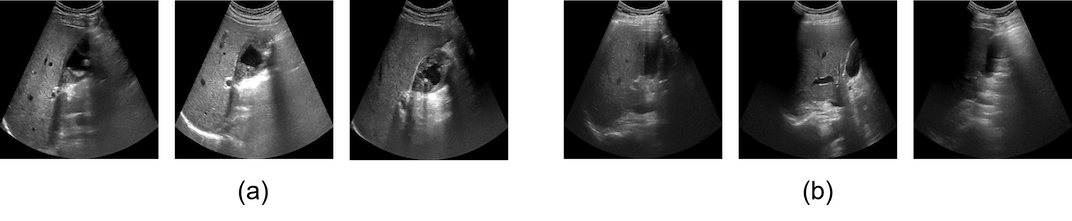
\includegraphics[width=0.9\linewidth]{figs/wsod/teaser.png}
    \caption[Low inter-class and high intra-class variability of GBC in USG data]{(a) Low inter-class variability. The first two GBs show benign wall thickening, and the third one shows malignant thickening. However, the appearance of the GB in all three images is very similar. (b) High intra-class variability. All three images have been scanned from the same patient, but due to the sensor's scanning plane, the appearances change drastically.}
    \label{wsod_fig:variability_teaser}
\end{figure}

\begin{figure}[t]
    \centering
    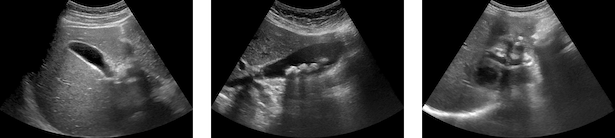
\includegraphics[width=\linewidth]{figs/non_reg_anatomy.png}
    \caption[Visualization of non-regular anatomy of the malignant gallbladders]{Normal, benign, and malignant \gb sample in \usg images, respectively (left to right). While normal or benign \gb have a regular, pear-shaped anatomy, a clear boundary is absent in the malignant \gb.}
    \label{fig:non_reg_anatomy}
\end{figure}


\subsection{Low Inter-Class and High Intra-Class Variability}
%
The manifestation of malignancy often occurs in a small part of the image, resulting in low inter-class variability, as most part of the images contain similar visual appearances. Also, as discussed earlier, the conflicting appearances in some of the benign and malignant wall thickening adds to the low inter-class variability. Simultaneously, USG images manifest significant variability in viewpoints for the same patient due to the handheld probe. This results in high intra-class variability, adding to the intricacies of accurate prediction for DNN models, as depicted in \cref{wsod_fig:variability_teaser}. The amalgamation of these challenges underscores the need for innovative solutions in GBC detection from USG images.

\begin{figure}[t]
    \centering
    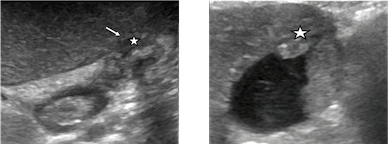
\includegraphics[width=0.8\linewidth]{figs/fasting.png}
    \caption[Effect of metabolic state on GB distension]{On left, the patient was in non-fasting state. On right, the patient was in fasting for 12 hours. Note the wall characteristics are much well appreciated in fasting state. Stars point to the focal thickening of the wall with adjacent liver infiltration. }
    \label{fig:fasting}
\end{figure}

\subsection{Non-regular Anatomy}
%
% Malignant GB usually exhibits non-regular anatomy, including a loss of interface with adjacent organs and irregular anatomical structure. \cref{fig:non_reg_anatomy} highlights the issue pictorially. The non-malignant GB in most cases demonstrate a clear anatomical pear-shaped structure. However, for malignant GBs, the entire GB is most cases is replaced by lesion or mass, making it difficult to even conclude the presence of a GB. 

The detection of gallbladder malignancy is further complicated by the non-regular anatomy typically associated with malignancy. Malignant gallbladders often showcase irregularities such as a loss of interface with adjacent organs and a distorted anatomical structure. \cref{fig:non_reg_anatomy} visually highlights this issue. In non-malignant cases, the GB typically exhibits a clear pear-shaped structure with distinct anatomical features. However, for malignant gallbladders, the entire gallbladder is frequently replaced by a lesion or mass, making it challenging to even identify the presence of a gallbladder in certain cases. Such non-regular anatomy further emphasizes the intricacies involved in distinguishing between malignant and non-malignant cases in USG images.

\subsection{Effect of the Metabolic State of the Patients}
%
If the patients are in fasting state, the gallbladder is well distended, and the abnormalities can be well detected. However, if the patient is not in fasting state, the contracted gallbladder adds to the difficulty of diagnosis. \Cref{fig:fasting} shows how acquiring the image samples after keeping the patient in 12-hour fasting helps in obtaining a better view of the gallbladder. Thus, it is important to obtain the data in the correct metabolic state to ensure the presence of adequate visual features in the captured images.

\subsection{Lack of Annotated Data}
%
%The absence of a well-annotated dataset poses another challenge for developing and training accurate DNN models for GBC detection, hindering progress in the field. Prior to our work, there was no public dataset with annotated USG images or videos for training the GBC detectors. 
The lack of a well-annotated dataset presents an additional hurdle in the development and training of accurate DNN models for GBC detection, impeding advancements in the field. Prior to our research, public datasets with annotated Ultrasound images or videos for training GBC detectors did not exist. The absence of comprehensive and annotated datasets significantly hampers the ability to train and optimize DNN models for the specific task of GBC detection, highlighting the need for dataset contributions and novel approaches involving training with a low volume of data in this domain.

\subsection{Challenges Addressed in this Work}
%
In this work, our developed techniques in Chapters 4--8 could solve the issues arising from the noises and artifacts such as acoustic shadows, bias to echogenic textures, small sized pathological regions, variation in appearance due to non-regular anatomy to a large extent in our data. To tackle the lack of annotated data, self-supervised representation learning has also been utilized. The issues related to operator and viewpoint variability largely affects the image-based GBC detectors. The use of video-based detectors could mitigate the effect of operator and viewpoint variability.

It is important to note that we have primarily addressed multiple issues of DNN-based malignant vs. benign GB  differentiation on single-center retrospective ultrasound data. Further, staging of malignancy, or differential diagnosis were not studied. A precise assessment of the methods in tackling acquisition shifts and their generalization performance requires more data from different centers, as single-center data only involves a few radiologists and a limited set of ultrasound apparatus. Due to the absence of publicly available data or other hospitals' data, we could not quantitatively assess the robustness and generalization performance for GBC detection, and noted it as a future research direction. However, it is important to note that the inherent issues such as noise, textures, and non-regular anatomy would remain constant for GBC ultrasound data from other centers. Additionally, we have demonstrated the generality and applicability of the developed methods on datasets for other diseases, such as breast cancer, COVID-19, and polyp detection, indicating the generalizability of the methods.

Furthermore, our data collection was from an apex tertiary care hospital in Northern India, which attends patients from different states, ethnicities, genders, and demographics. The patients are not localized to the region of the hospital, and far-off patients also visit for care. This ensures a high degree of patient variability in our data. Thus, we expect our techniques to perform robustly. Nonetheless, some performance drop is expected while applying the models on unseen data from other centers due to operator and equipment variability. %Especially image-based detection models tend to be more susceptible to acquisition shift arising from operator variability.

%In this work, we have primarily addressed multiple issues on single-center retrospective patient data. The use of techniques such as focused regions-of-interest, smoothing-based curriculum, multi-scale features, second order feature attention, global-local features, could solve the issues arising from the noises and artifacts such as acoustic shadows, echogenic textures, non-regular anatomy, and data variability to a large extent in our data. To tackle the lack of annotated data, self-supervised representation learning has also been utilized. The issues related to operator and viewpoint variability largely affects the image-based GBC detectors. The use of video-based detectors could mitigate the effect of operator and viewpoint variability. 

%However, a precise assessment of the methods in tackling operator variability and acquisition shifts requires more data from different centers, as single-center data only involves a few radiologists and a limited set of ultrasound apparatus. Due to the absence of publicly available data or other hospitals' data, we could not quantitatively assess the robustness and generalization performance for GBC detection, and noted it as a future research direction.

%However, it is important to note that the inherent issues such as noise, textures, and non-regular anatomy would remain constant for GBC ultrasound data from other centers. Additionally, we have demonstrated the generality and applicability of the developed methods on datasets for other diseases, such as breast cancer, COVID-19, and polyp detection, strongly indicating the generalizability of the methods.

%Furthermore, our data collection was from an apex tertiary care hospital in Northern India, which attends patients from different states, ethnicities, genders, and demographics. The patients are not localized to the region of the hospital, and far-off patients also visit for care. This unique characterization ensures a high degree of patient variability in our data. Thus, we expect our techniques to perform robustly. Nonetheless, some performance gap due to acquisition shift arising from operator and equipment variability is expected.